\documentclass[prd,amsmath,amssymb,floatfix,nofootinbib,preprintnumbers,twocolumn]{revtex4}%showpacs,superscriptaddress
\usepackage[latin1]{inputenc}
\usepackage{amsmath}
\usepackage{amsfonts}
\usepackage{hyperref}
\usepackage{amssymb}
\usepackage{graphicx,multirow}
\usepackage{appendix}
\usepackage{dcolumn}
\usepackage{caption}
\usepackage{subfigure}
\usepackage{float}
\usepackage{bm}
\usepackage{latexsym}
\usepackage{epsfig}
\usepackage{graphicx,color}


\newcommand{\beq}{\begin{equation}}
\newcommand{\eeq}{\end{equation}}
\newcommand{\beqry}{\begin{eqnarray}}
\newcommand{\eeqry}{\end{eqnarray}}

\graphicspath{{figs/}}

\begin{document}

\title{Exact Q/U to E/B conversion of CMB polarization maps in the presence of a mask}
\author{Aditya Rotti\footnote{aditya@fsu.edu}, Kevin Huffenberger\footnote{huffenbe@physics.fsu.edu}}
\affiliation{Department of Physics, Florida State University, Keen Physics Building, 77 Chieftan Way, Tallahassee, Florida, U.S.A.}

\date{\today}

\begin{abstract}
The CMB photons are polarized and one of the main aims of future CMB missions will be to measure the CMB polarization sky with a precision which matches the temperature anisotropy measurement. However the measured CMB polarization sky, will still need to be masked to avoid the contamination due to galactic sources of polarized emission. While the CMB polarization is measured in terms of the Stokes Q and U parameters, it is more convenient to work in the E/B representation of the CMB polarization which has desirable properties under coordinate transformations. Masking however makes the decomposition of the measured Stokes parameters to E/B fields non-ideal. Specifically masking introduces some pseudo mixing of power between E-mode and B-mode maps. We present a method which allows an exact evaluation of the E/B maps of the polarized CMB sky on a masked sky, which overcomes this mixing problem.
\end{abstract}

\maketitle



\section{Introduction}

The CMB polarization is measured in terms of the Stokes Q and U parameters. These measurements can be combined to form the complex spin 2 polarization field as follows,
%
\beqry
_{\pm 2}X(\hat{n}) &=& Q(\hat{n}) \pm i U (\hat{n}) \nonumber \\ 
                                 &=& \sum_{\ell m}  {_{\pm 2}}X_{\ell m}  {_{\pm 2}}Y_{\ell m} (\hat{n})
\eeqry
%
Given this spin-2 field, it is possible to define two scalar fields denoted by $E(\hat{n}) $ and $B(\hat{n}) $, which are related to $_{\pm 2}X(\hat{n})$ through the following expression,
%
\beqry \label{ebdef}
E(\hat{n}) = -\frac{1}{2} \big[ \bar{\eth}^2 _{+ 2}X(\hat{n})  +  \eth^2 _{- 2}X(\hat{n}) \big] \,, \\
B(\hat{n}) = -\frac{1}{2i} \big[ \bar{\eth}^2 _{+ 2}X(\hat{n})  -  \eth^2 _{- 2}X(\hat{n}) \big] \,,
\eeqry
%
where $\eth$ and $\bar{\eth}$ denote the spin raising and lowering operators respectively. $E$ and $B$ fields are spin-0 fields similar to the temperature anisotropies. These operators are known to have the following properties,
%
\beqry \label{spinopylm}
\eth _s Y_{lm}(\hat{n}) &=& \sqrt{(\ell-s)(\ell+s+1)} _{s+1} Y_{lm}(\hat{n}) \,, \\
\bar{\eth} _s Y_{lm}(\hat{n}) &=& -\sqrt{(\ell+s)(\ell-s+1)} _{s-1} Y_{lm}(\hat{n}) \,, 
\eeqry
%
where $_s Y_{lm}(\hat{n}) $ are the spin spherical harmonics.

Using Eq.\ref{ebdef} and the properties of the spin raising and lowering operators given in Eq.~\ref{spinopylm} it can be shown that the $E/B$ fields are given by the following set of equations,
%
\beqry
E(\hat{n})  &=& \sum_{\ell m} e_{\ell m} \sqrt{\frac{(\ell+2)!}{(\ell-2)!}} Y_{\ell m} (\hat{n}) \,, \\
B(\hat{n})  &=& \sum_{\ell m} b_{\ell m} \sqrt{\frac{(\ell+2)!}{(\ell-2)!}} Y_{\ell m} (\hat{n}) \,,
\eeqry
%
where the harmonic coefficients of the $E/B$ fields are related to the spin harmonic coefficients of the polarization field through the following equations,
%
\beqry
e_{\ell m} = -\frac{1}{2} \big[ _+ X_{\ell m} + _- X_{\ell m} \big] \\
b_{\ell m} = -\frac{1}{2i} \big[ _+ X_{\ell m} - _- X_{\ell m} \big] 
\eeqry
%
\section{Masking and $E/B$ decomposition}

Portions of the measured polarization sky need to be masked in order to ensure that emission from the Milky Way do not contaminate the cosmological signal. In such a case, the $E/B$ fields need to be constructed from a masked polarization field,
%
\beqry \label{ebdef}
\tilde{E} = -\frac{1}{2} \big[\bar{\eth}^2 (W{_{+ 2}}X)  +  \eth^2 (W {_{- 2}}X) \big] \,, \\
\tilde{B} = -\frac{1}{2i} \big[ \bar{\eth}^2 (W{_{+ 2}}X)  -  \eth^2 (W{_{- 2}}X)\big] \,,
\eeqry
%
\noindent where $W$ denotes the mask and $\tilde{E}/\tilde{B}$ represent the scalar fields recovered from masked polarization maps.

As discussed in appendix, it can be shown that the spin operators follow the product rule. Using this fact it can be shown that the above equation can be expressed in the following form,
%
\beqry
&&\tilde{E} = -\frac{1}{2}W( \bar{\eth}^2 _{+ 2} X  + \eth^2 _{- 2}X ) \\
 &-& \frac{1}{2} (_{+ 2} X  \bar{\eth}^2 W  + _{- 2}X \eth^2 W ) - (\bar{\eth} W  \bar{\eth} _{+ 2} X + \eth W  \eth  _{- 2} X ) \nonumber \\
 &&\tilde{B} = -\frac{1}{2i}W( \bar{\eth}^2 _{+ 2} X  - \eth^2 _{- 2}X ) \\
 &-& \frac{1}{2i} (_{+ 2} X  \bar{\eth}^2 W  -  _{- 2}X \eth^2 W ) + i (\bar{\eth} W  \bar{\eth} _{+ 2} X - \eth W  \eth  _{- 2} X ) \nonumber
\eeqry
%
The above set of equations can be cast in the following revealing form,
%
\beqry
\tilde{E} &=& WE - [~\mathrm{ Re}(_{+ 2} X  \bar{\eth}^2 W)  +~ 2 \mathrm{ Re}( \bar{\eth} W  \bar{\eth} _{+ 2} X )]\,, \\
\tilde{B} &=& WB -  [\mathrm{Img}(_{+ 2} X  \bar{\eth}^2 W)  + 2\mathrm{Img}(\bar{\eth} W  \bar{\eth} _{+ 2} X)] \,,
\eeqry
%
Therefore we can now write down expression for the masked true $E/B$ fields, in terms of $\tilde{E}/\tilde{B}$ and the residual terms,
%
\beqry \label{res-core-eb}
WE &=& \tilde{E}  +  ~\mathrm{Re}[_{+ 2} X (\bar{\eth}^2 W) +  2(\bar{\eth} W  \bar{\eth} _{+ 2} X)] \\
WB &=& \tilde{B}  + \mathrm{Img}[_{+ 2} X (\bar{\eth}^2 W) +  2(\bar{\eth} W  \bar{\eth} _{+ 2} X)] 
\eeqry
%

The spin lowering operations on the mask and on the polarization field are easily evaluated in harmonic space and the relevant terms in the above equation can be expressed in terms of harmonic coefficients as follows,
%
\beqry
\bar{\eth} W(\hat{n}) &=&\sum_{\ell m} - w_{\ell m} \sqrt{\ell(\ell+1)}  {_{-1}} Y_{\ell m}(\hat{n}) \,, \\
\bar{\eth}^2 W(\hat{n}) &=& \sum_{\ell m} w_{\ell m} \sqrt{\frac{(\ell+2)!}{(\ell -2)!}}  {_{-2}} Y_{\ell m}(\hat{n})  \,, \\
\bar{\eth} {_{2}}X(\hat{n}) &=&\sum_{\ell m} - {_{2}}X_{\ell m} \sqrt{(\ell+2)(\ell-1)}  {_{1}} Y_{\ell m}(\hat{n}) \,,
\eeqry
%
where $w_{\ell m}$ and $_{2}X_{\ell m}$ are the spherical harmonics of the mask and the unmasked polarization field. Here one might be concerned with the fact that there appears derivatives of the unmasked polarization field, which might propagate foreground contamination to the constructed $E/B$ maps. However note that the product of the polarization field or its derivatives is always with terms which involve derivatives of the mask.  The derivatives of the mask is zero everywhere except on the edges of the mask, hence the leakage  of the foregrounds into the constructed $E/B$ can be completely controlled by properly tailoring the mask, such that the derivatives of the mask are non-vanishing only in regions where the the mask is absent. Also note that the mask needs to be in proper apodized form which is important to ensure that the power spectrum in the mask is band limited.  The apodization is also critical in ensuring that the mask derivatives are well defined. 

\section{A toy example}

Though the above description was carried out keeping in mind that the polarization maps need to be masked, it is equally valid for for a case when the polarization field is multiplied by an arbitrary spin 0 field. We show multiplying the polarization field by a simple dipolar field, does induce $E/B$ mixing. We then evaluate the residual terms arising due to this the dipolar field and show that on subtracting the residual, you do recover the masked true $E/B$ fields with power spectrum fully consistent with the input $E/B$ spectrum.

To carry out this exercise we generate polarization field with E-mode power spectrum given by some fiducial model and we assume zero B-mode power. Hence after residual subtraction, it is expected that the residual subtracted B-mode map have power which is identical to the input  power spectrum of the masked input B-mode map (Note : This should be in principle zero, but is has some non-zero value only due to numerical accuracy). 

\begin{figure}[!h]
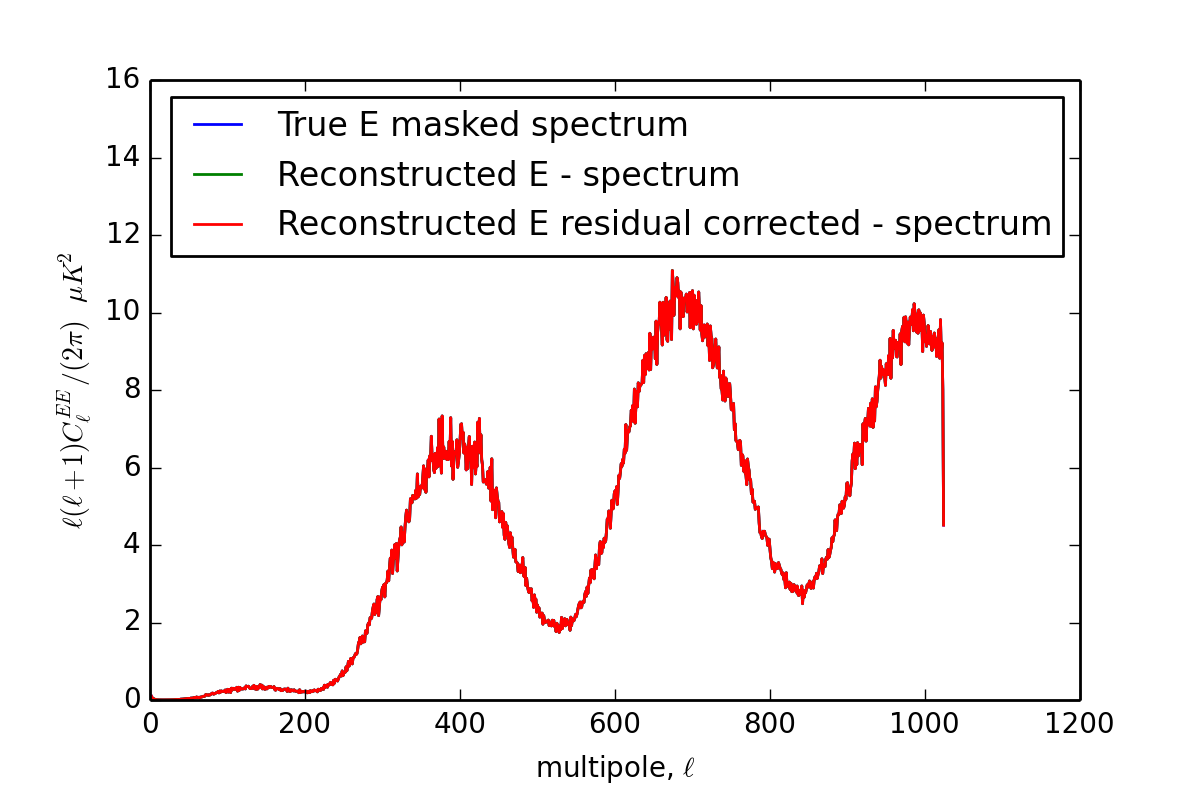
\includegraphics[scale=0.6]{clee-compare.png}
\caption{This figure depicts the power spectrum of the masked E-mode sky for the true E-field masked, the reconstructed E-field and the reconstructed E-field corrected for the residual due to the mask. In this figure they all lie on top of each other. Look at the difference figure which depict the minor differences.}
\end{figure}

\begin{figure}[!h]
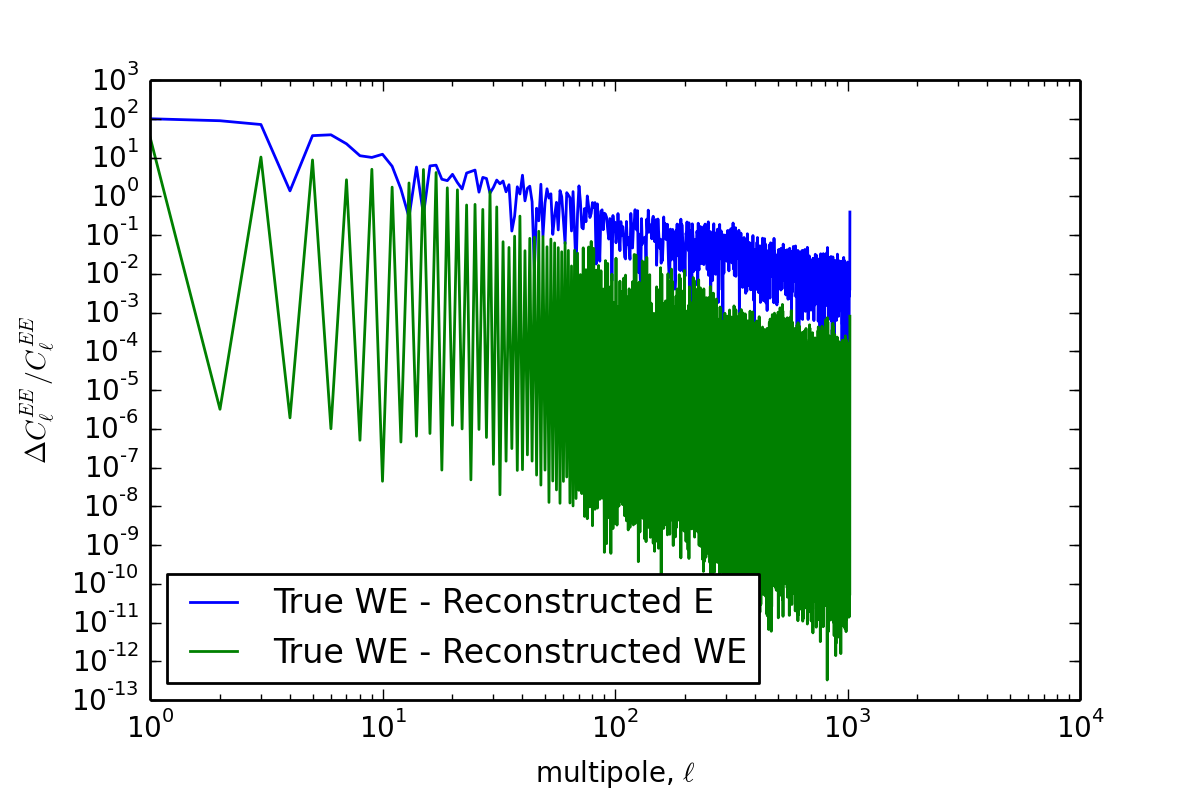
\includegraphics[scale=0.6]{diffclee.png}
\caption{This figure depicts the relative difference between the reconstructed B-mode spectrum and the true E-mode spectrum. These differences are not visible in the plots of the spectrum themselves. However note that the residual subtraction, does reduce the distance between the true E-mode spectrum and the reconstructed E-mode spectrum.}
\end{figure}

\begin{figure}[!h]
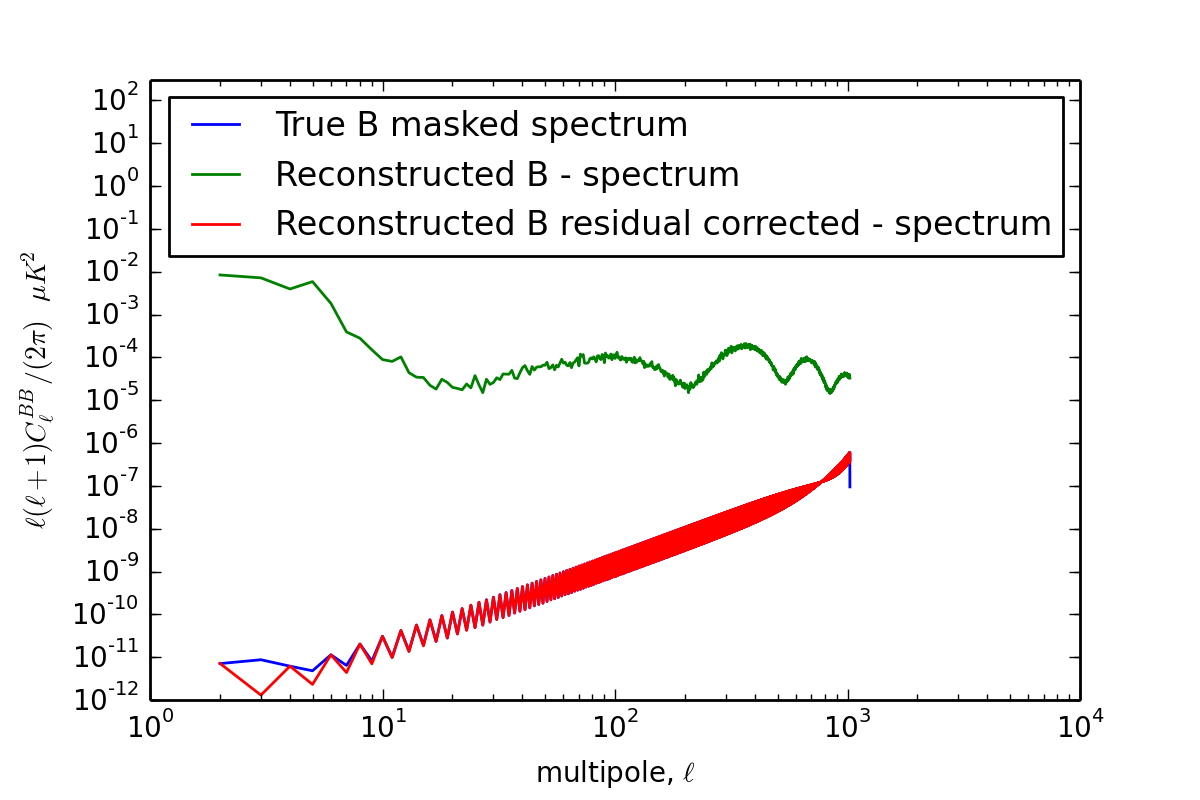
\includegraphics[scale=0.6]{clbb-compare.png}
\caption{This figure depicts the power spectrum of the masked B-mode sky for the true B-field masked (blue), the reconstructed B-field (green) and the reconstructed B-field(red) corrected for the residual due to the mask. Note the excess power seen in the B-mode map recovered from the masked polarization sky, this is sourced by masking the polarization maps. More importantly note that on residual subtraction (See Eq. 17), we do recover the power spectrum which matches the true B mode power spectrum.}
\end{figure}

\section{Robustness against foregrounds}

In Eq.\ref{res-cor-eb} there appears a term which requires the spin raising/lowering operators to operate on the unmasked polarization field. Though this is not a problem in the case where the CMB maps have no foregrounds, it is most likely to cause leakages to to other portions of the sky in the presence of foregrounds. To over come this problem and make the E/B reconstruction more robust in the presence of foregrounds, we multiply Eq.\ref{res-cor-eb} and use the fact that the spin raising lowering operation obey the product rule, to recast the equations in the following form.

%
\beqry
W^2E &=& W\tilde{E}  +  ~\mathrm{Re}[W_{2} X (\bar{\eth}^2 W)] \nonumber \\ &+&  2\mathrm{Re}[\bar{\eth} W  \bar{\eth} (W_{ 2} X) - 2\bar{\eth} W  \bar{\eth}W _{ 2} X] \\
W^2B &=& W\tilde{B}  + \mathrm{Img}[W_{ 2} X (\bar{\eth}^2 W)] \nonumber \\ &+&  2 \mathrm{Img}[\bar{\eth}W\bar{\eth}(W_{ 2} X) - 2\bar{\eth} W  \bar{\eth}W _{ 2} X] 
\eeqry
%

\section{Conclusions}

We have formulated an exact conversion of $Q/U$ to $E/B$ maps in the presence of a mask. It has been shown to work extremely well when we use a dipolar field which has azimuthal symmetry as a mask. Ongoing work to show that  this will work for an arbitrary field and then finally to a practical polarization mask with proper apodization.

\appendix
\section{Product rule for spin operators}

A field is said to have spin s if it obeys the following transformation property, under the rotation of the coordinate system at a point by angle $\theta$,
%
\beq
_s f' \rightarrow e^{is\theta} {_s} f
\eeq 
%
Using this property it is easy to show that the product of two fields with spins $s_1$ and $s_2$ respective has spin $s_1 + s_2$.
%
\beq
_{s_1 +s_2=s}f ={_{s_1}} g {_{s_2}}h
\eeq
%
The spin raising operator $\eth$ can be written down as follows,
%
\beq
\eth {_{s}}f(\theta,\phi) = -\sin^s\theta \bigg[ \frac{\partial}{\partial \theta} + \frac{i}{\sin\theta} \frac{\partial}{\partial \phi} \bigg] \sin^{-s}\theta {_s}f(\theta,\phi) 
\eeq
%
Using this definition it can be shown that,
%
\beq
\eth {_{s}}f = {_{s_2}}h~ \eth {_{s_1}}g  + {_{s_1}}g~\eth{_{s_2}}h
\eeq
%


\end{document}
